\documentclass[a4paper,11pt]{article}
\hyphenpenalty 10000
\usepackage[utf8]{inputenc}
%\usepackage[T1]{fontenc}
\usepackage{amsmath,amssymb}
\usepackage[english,french]{babel}
\usepackage[pdftex]{graphicx}
%\usepackage[options]{mcode}
\usepackage{textcomp}
\usepackage{array}
\usepackage{subfig}
\usepackage[left=2.5cm, right=2.5cm, bottom=2.5cm, top=2.5cm]{geometry}
\usepackage{float}
\usepackage{multicol}
\usepackage{tabularx}
\usepackage{fancybox}
\usepackage{color}


\usepackage{color} % gestion de différentes couleurs

\definecolor{linkcolor}{rgb}{0,0,0.6}% définition de la couleur des liens pdf
\usepackage[ pdftex,colorlinks=true,
pdfstartview=FitV,
linkcolor= linkcolor,
citecolor= linkcolor,
urlcolor= linkcolor,
hyperindex=true,
hyperfigures=false]
{hyperref} % fichiers pdf 'intelligents', avec des liens entre les références, etc.

\usepackage{fancyhdr} % entêtes et pieds de pages personnalisés 
\pagestyle{fancy}
\fancyhead[L]{\scriptsize \textsc{Etude théorique de la translocation de
biomolécules à travers un nanopore}}
\fancyhead[R]{\scriptsize \textsc{Menais Timothée}}
\fancyfoot[C]{ \thepage} 

\begin{document}



% Pour faciliter la mise en forme de la page du titre, on supprime l'indentation automatique en début de paragraphe
\setlength{\parindent}{0pt}

% Pas d'en-tête ni de pied pour la première page
\thispagestyle{empty}


\includegraphics[height=2cm]{phelma.jpg} \hfill 
\includegraphics[height=2cm]{cea2.png} \hfill 
\includegraphics[height=2cm]{ujf.jpg}

\vspace{0.5cm}

\begin{tabularx}{\textwidth}{@{} l X l @{} }
{\sc Master  2R EP} & & Rapport de stage 2012 \\
{\it Grenoble INP, PHELMA} & & Menais Timothée \\

\end{tabularx}

\begin{center}

\vspace{1.5cm}

\rule[11pt]{5cm}{0.5pt}

\textbf{\huge Etude théorique de la translocation de
biomolécules à travers un nanopore}

\rule{5cm}{0.5pt}

\vspace{1.5cm}

\parbox{15cm}{\small
\textbf{Abstract} : \it Rapport de stage, M2R EP, Timothée Menais, 2011-2012.

\vspace{0.5cm}
\rm On verra plus tard pour la présentatin de l en tete.
} %fin de la commande \parbox du résumé


\vspace{0.5cm}

\parbox{15cm}{
\textbf{Mots clés : \it ADN, Graphène, Dynamique moléculaire, Physique statistique.} }%fin de la commande \parbox des mots clefs

\vspace{0.5cm}

\parbox{15cm}{
Stage encadré par :

{\bf Dr Arnaud Buhot }

\href{mailto:	arnaud.buhot@cea.fr }{\tt 	arnaud.buhot@cea.fr }  / tel: ++33 438 78 38 68

%{\bf Dr Ulrich Keyser}

%\href{mailto:	ufk20@cam.ac.uk}{\tt 	ufk20@cam.ac.uk} / tel: +44 (0)1223 337272

Groupe Théorie

Structures et Propriétés d'Architectures Moléculaires

Institut Nanoscience et Cryogénie
{\it 

17 rue des Martyrs
38054 Grenoble cedex 9
France}

\url{http://inac.cea.fr/spram/Phocea/Vie_des_labos/Ast/ast_groupe.php?id_groupe=397}
} %fin de la commande \parbox encadrant / laboratoire d'accueil

\vspace{1cm}



\includegraphics[height=1.8cm]{spram.jpg} \hspace{0.3cm}

\includegraphics[height=1.8cm]{inac.jpg}

\end{center}


\begin{flushright}
\today
\end{flushright}

\vfill
\hfill 

% Pas d'entête ni de pied pour la page de sommaire



\setlength{\parindent}{10pt}

\newpage



\section{Translocation à travers une membrane fixe}



\subsection{Préparation à la translocation}

\subsubsection{Définition de la membrane}

Bien que d'autres cristaux bidimensionnels existent, le graphène reste le candidat principal pour le séquençage en utilisant des nanopores dans des membranes fines. Nous avons donc considéré un modèle de mambrane proche de ce dernier.
Afin de modéliser la membrane à travers laquelle notre polymère va effectuer une translocation, nous avons choisis de respecter les dimensions relatives  entre le graphène et l'ADN. Un réseau hexagonal de paramètre de maille $\frac{\sigma}{2}$ a été généré (voir figure \ref{reseau}. Le plan de graphène est suffisamment étendu pour qu'avec des conditions aux limites périodiques (pour simuler un plan infini), le polymère le plus grand utilisé ne puisse jamais se retoucher lui même, soit 5488 grains. Cette étendue importante implique que les atomes de notre membrane seront les atomes majoritaires.

\begin{figure}[H]
\begin{center}
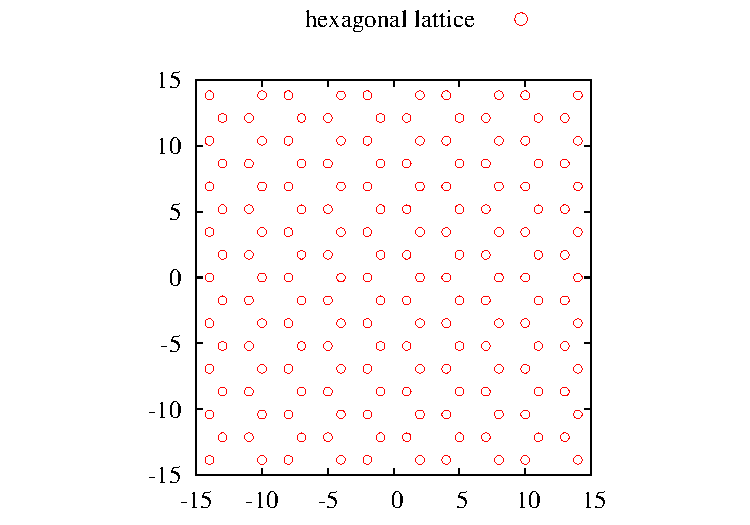
\includegraphics[width=0.6\textwidth]{lattice.pdf} 

\caption{Notre réseau héxagonal}
\label{reseau}
\end{center}
\end{figure}

Le réseau est ensuite amputé en son centre de tous les grains situés dans un rayon fixé pour créer le pore. Dans ce chapitre, les grains de la membranes sont fixes, les équations du mouvement ne sont pas intégrées pour la membrane, elle n'existe qu'à travers l'intéraction avec le polymère par des potentiels stériques de type Lennard-Jones. Afin d'éviter que le notre polymère ne pénétre entre les grains de notre membrane, nous avons choisi $\sigma_{ij}=sigma$ pour toute intéraction avec un grain de la chaîne du polymère et $\sigma_{ij}=1.25\sigma$ pour un grain latéral. Cette valeur est supérieur à l'espacement entre grains de la membrane. Physiquement, dans le cas du graphène ces tailles correspondent à la taille des orbitales atomiques de type $\pi$ du graphène avec lesquelles le polymère intéragit.


\subsubsection{Polymère greffé et configurations initiales}

Une fois notre système défini, nous devons le préparer pour étudier la translocation. Pour cela, nous allons créer des configurations initiales indépendantes qui seront le prélude à la translocation. 



La translocation peut se dérouler dans différents contextes. Elle peut être due uniquement aux fluctuations thermiques, on parle alors de translocation non biaisée, ou être pilotée par une force extérieure, on parle alors de translocation forcée (driven translocation). Les forces extérieures peuvent être de natures variées, on citera notamment l'utilisation de champs électriques (électrophorèse), de gradients de potentiels chimiques, de flux imposé sur le solvant, ou encore l'emploi de pinces optiques \cite{keyser}.\\

Le temps de translocation dépend alors fortement de la taille du polymère et de la force appliquée, d'une façon générale on peut définir des lois d'échelles:

\begin{eqnarray}
\tau = N^\alpha f^{-\delta}
\label{tau}
\end{eqnarray}

 Le but du stage est de déterminer les valeurs de $\alpha$ et $\delta$, appelés exposants critiques, dans les différentes limites possibles. On basera l'échelle de force en unités de Lennard-Jones à partir de la valeur de $\frac{\epsilon}{b}$.\\

Nous allons dans un premier temps calculer la forme de la barrière d'énergie franchie par le polymère lors de la translocation. Pour cela, nous devons dans un premier temps calculer la probabilité de distribution d'un polymère idéal greffé à une paroi. La chaîne idéale présente comme conditions aux limites, la non pénétration des monomères à travers la paroi. On note $P(\textbf{r},\textbf{r}_0,n)$ la probabilité de trouver le $n$-ième monomère en position $\textbf{r}$, pour $n \gg 1$, le premier monomère étant greffé en $\textbf{r}_0$. $P_0$ est la distribution calculé précédemment pour un polymère idéal libre.

\begin{eqnarray}
P_0(\textbf{r},\textbf{r}_0,n)=\left(\frac{3}{2\pi n b^2}\right)^\frac{3}{2}\exp\left(-\frac{3(\textbf{r}-\textbf{r}_0)^2}{2 n b^2}\right)
\end{eqnarray}

A l'instar de nombreux problèmes d'électromagnétisme ou de mécanique des fluides, on utilise la méthode des images miroirs afin de déterminer $P(\textbf{r},\textbf{r}_0,n)$. En effet, on a:

\begin{eqnarray}
P(\textbf{r},\textbf{r}_0,n) \propto P_0(\textbf{r},\textbf{r}_0,n)-P_0(\textbf{r},-\textbf{r}_0,n)
\end{eqnarray}

Dans le cas idéal, la probabilité de distribution du monomère de queue est à variables séparables. En posant $\textbf{r}_0= \epsilon y$ avec $\epsilon \ll 1$, un développement limité au premier ordre donne:

\begin{eqnarray}
P(\textbf{r},\textbf{r}_0,n) \propto \left(\frac{3}{2\pi n b^2}\right)^\frac{3}{2} \left(\frac{6 y \epsilon}{n b^2}\right)\exp\left(-\frac{3\textbf{r}^2}{2 n b^2}\right)
\end{eqnarray}

Pour le cas non idéal, les termes supplémentaires introduits dans $P_0$ ne permettent pas de séparer les variables et d'obtenir une expression analytique.


\begin{figure}[H]
\begin{minipage}{0.45\linewidth}
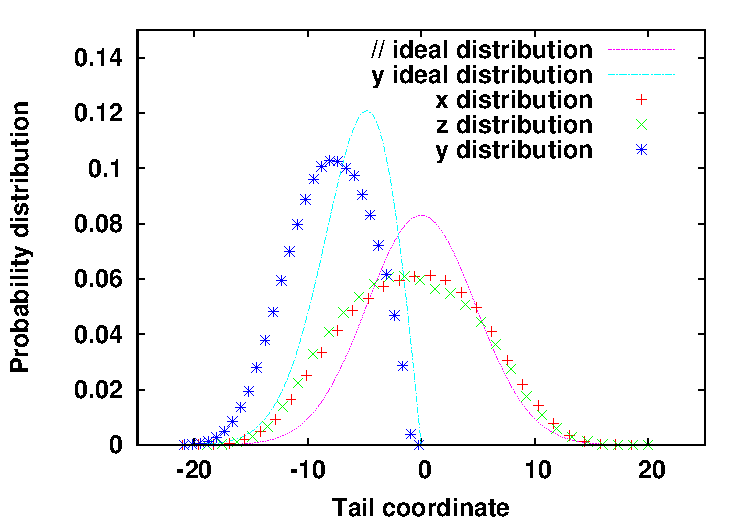
\includegraphics[width=1.2\textwidth]{probdistribution.pdf}

\end{minipage}\hfill
\begin{minipage}{0.45\linewidth}
\caption{Probabilité de distribution théorique du monomère de queue pour un polymère idéal et résultats numériques pour un polymère à monomères durs (N=35). Parallèlement à la membrane, la distribution gaussienne idéale est aplatie au centre à cause de la zone d'exclusion des autres monomères. De même pour la direction perpendiculaire, le pic maximum est repoussé par la présence d'autres monomères. Dans les deux cas, l'éloignement maximal n'est pas modifié car le cas idéal correspond déjà à des chaînes étirées sans superpositions de monomères. }
\label{polagainstwall}
\end{minipage}
\end{figure}


Afin d'aborder la translocation, nous avons du créer des configurations indépendantes de polymères à l'équilibre, juste avant l'application d'une force. Lors de ce processus de génération, nous avons laisser le polymère évoluer librement en fixant une extrémité au centre du pore. L'étude des coordonnées du grain de queue nous a permis d'évaluer l'influence des volumes exclus, comme le montre la Figure \ref{polagainstwall}.


La probabilité de distribution du polymère accolé à une membrane permet, à partir de la fonction de partition stérique, $Z_S(n)= \int_{y>0} P(\textbf{r},\textbf{r}_0,n) \textbf{dr}$, de calculer l'énergie libre d'origine entropique d'un tel système. Dans la limite $n \gg 1$, le premier terme non nul du développement limité impose la loi d'échelle: $Z_S(n) \propto n^{-1/2}$. Pour un polymère de $N$ monomères en cours de translocation, lors du passage du $n$-ième monomère, on obtient la valeur de l'énergie libre en prenant en compte les effets entropiques de part et d'autre de la membrane:
\begin{eqnarray}
F(N,n)= -k_BT\ln\left(Z_S(n)Z_S(N-n)\right)= \frac{1}{2} k_BT \ln \left(n(N-n)\right) +cste
\end{eqnarray}

Cette barrière d'énergie à franchir au cours de la translocation peut être altérée en appliquant une différence de potentiel, chimique ou électrique, ou encore en appliquant directement une force sur la chaîne. La Figure \ref{energiebarrier} montre cette barrière d'énergie.
\begin{figure}[H]
\begin{center}
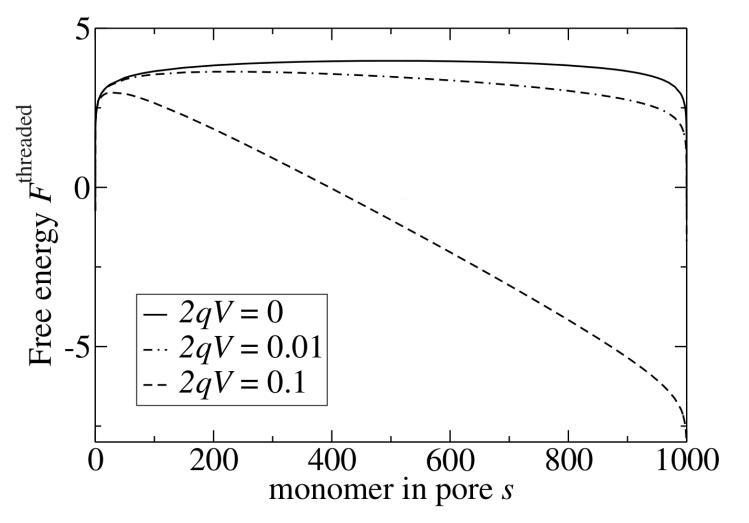
\includegraphics[width=0.4\textwidth]{transelec.jpg} 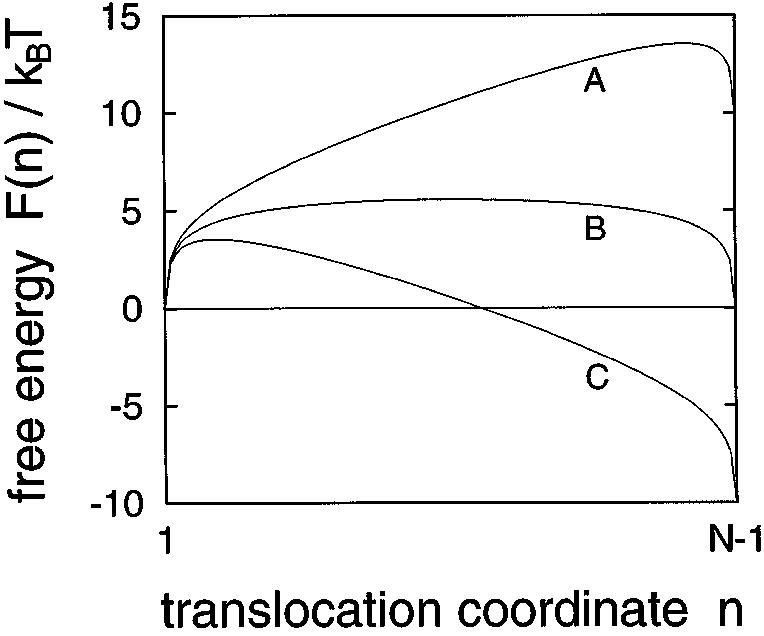
\includegraphics[width=0.28\textwidth]{transpotchim.jpg}

\caption{Modification de la barrière entropique par une différence de potentiel électrique (à gauche \cite{these}) et de potentiel chimique (à droite \cite{sung}). A: différence de potentiel opposée à la translocation, B: différence de potentiel nulle, C: différence de potentiel favorable.}
\label{energiebarrier}
\end{center}
\end{figure}

 Lors de la translocation non biaisée, la barrière d'énergie est utilisée pour résoudre l'équation de Smoluchowski, qui va permettre de déduire $\tau \propto N^{1+2\nu}$ comme limite inférieure. Le cas non biaisé n'a pas été étudié. Le lecteur intéressé trouvera démonstrations et explications dans l'article de revue de Milchev \cite{milchev}.
 
 Pour la translocation forcée, l'application d'une force bouleverse l'hypothèse de l'équilibre thermodynamique local utilisée pour évaluer $\tau$ dans le cas non biaisé. Plusieurs modèles hors équilibre sont présentés dans l'article de J. L. A. Dubbeldam et collaborateurs \cite{traction}. Nous retenons de la lecture de cet article que pour la dépendance en $N$, ils s'attendent à une transition de $\tau \propto N^{2\nu}$ à $\tau \propto N^{1+\nu}$ lorsque la force augmente. En ce qui concerne la dépendance en $F$, ils s'attendent à une transition de $\tau \propto F^{-1}$ à $\tau \propto F^{(1/\nu)-2}$ lorsque la taille de la chaîne diminue.



\subsubsection*{Translocation à travers un pore large}

Dans un premier temps, nous avons considéré une membrane fixe munie d'un nanopore large. Le nanopore est créé en supprimant 54 grains au centre. L'extrémité du polymère est alors tirée par l'ajout d'une force perpendiculaire à la membrane et d'amplitude modulée sur 3 ordres de grandeurs, de 0.1 à 100. Un cylindre de sécurité est implanté dans le code pour vérifier que le pore est toujours peuplé. Lorsque ce n'est plus le cas, nous vérifions si le polymère a terminé sa course du coté cis ou du coté trans. En effet, pour de faibles forces, le polymère peut dans certaines simulations, ne pas effectuer la translocation.\\

Trois polymères ont été étudiés, ils présentent 8, 16 et 32 monomères. A l'instar des prédictions de J. L. A. Dubbeldam et collaborateurs \cite{traction}, nous observons deux régimes distincts caractérisant la dépendance de la loi d'échelle avec la force. En effet, on observe à forces faibles (excepté pour $N=8$) et intermédiaires un comportement tel que $\tau \propto 1/F$. Pour des forces plus élevées, on trouve une loi d'échelle avec un exposant plus élevé ($\tau \propto F^{-0.74}$ pour N=8) Cet exposant plus élevé montre la transition vers $\tau \propto F^{(1/\nu) -2}$. La valeur plus faible qu'attendue peut être attribuée aux effets de taille finie et à l'amplitude de la force qui n'est pas assez élevée. De plus la transition entre les régime semble apparaitre plus tôt pour les $N$ faibles, contrairement à la prédiction de J. L. A. Dubbeldam et collaborateurs \cite{traction}. Cette différence pourrait venir du fait que nous tractons notre polymère (force en bout de chaîne), alors que dans leur cas, une différence de potentiel est appliquée (force au sein du pore). La Figure \ref{holebigger} permet de mieux visualiser ces régimes. En ce qui concerne l'évolution de $\tau$ avec $N$, on trouve un exposant de 1.78 pour les forces imposées de 9 et 20, et 1.69 pour 80. Ces valeurs sont proches du cas $\tau \propto N^{(1+\nu)}$ attendu pour les forces importantes.

Dans le cas $N=8$, nous observons un décrochement de pente. Ceci se produit lorsque la force est faible et pour une chaîne très courte. L'impulsion initiale donnée par le mouvement brownien rejette nombre de configurations (d’où une forte diminution du nombre de translocation réussies), celles conservées ayant une grande impulsion non naturelle dans le sens de la translocation, diminuant artificiellement $\tau$. Cette rupture de pente nous semble donc être un effet de taille finie.

Exercer des forces plus faibles nous ferait perdre beaucoup trop d'événements. Afin de balayer de larges domaines, il pourrait être intéressant de travailler, comme cela peut être fait expérimentalement à vitesse de traction imposée (la force n'est alors plus constante).

\begin{figure}[H]
\begin{center}
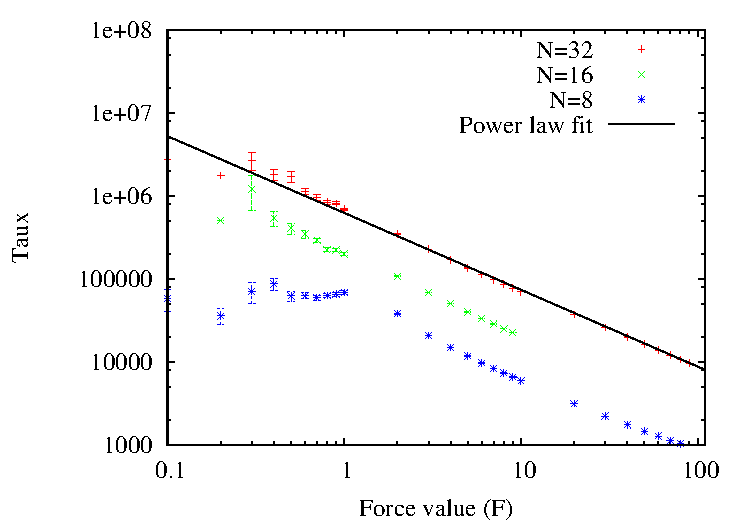
\includegraphics[width=0.48\textwidth]{translocfholebigger.pdf} 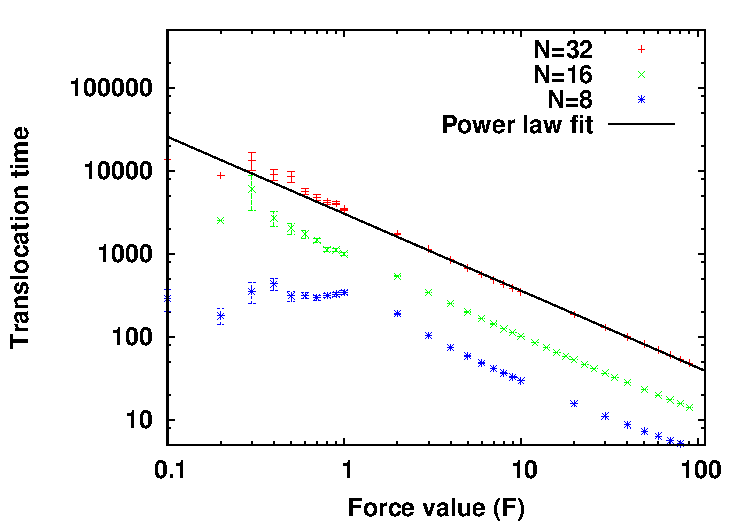
\includegraphics[width=0.48\textwidth]{translocholebigger.pdf}

\caption{Lors de la translocation à travers un pore large, on distingue deux régimes, une décroissance de $\tau \propto 1/F$ suivit d'une augmentation de l'exposant critique quand $F$ devient suffisamment grande. La rupture de pente du cas $N=8$ est imputée à des effets de taille finie. On trouve bien des valeurs proches de $\tau \propto N^{1+\nu}$ pour la dépendance en N.}
\label{holebigger}
\end{center}
\end{figure}

Afin de ralentir la translocation, enjeu clé du séquençage, nous allons maintenant étudier l'influence d'un nanopore plus étroit. En quoi le frottement important induit par le pore va-t-il modifier les lois d'échelle trouvées précédemment?


\subsubsection*{Translocation à travers un pore étroit}
Nous étudions dorénavant l'effet d'une membrane fixe munie d'un nanopore étroit qui va induire un frottement plus important. Le nanopore est créé en supprimant uniquement 24 grains au centre cette fois ci. Le pore a été choisi suffisamment étroit pour empêcher les monomères de passer de front, ils devront se déformer pour permettre le passage du grain latéral, plus volumineux.\\

Encore une fois, nous observons les deux régimes précédents. Cependant la frontière semble apparaitre plus tard à cause du frottement, ce qui diminue la force effective appliquée sur le polymère ($F_{eff}=F-\epsilon _{pore})$. Les mêmes lois d'échelles sont observées à forte force ( $\tau \propto 1/F$ puis $\tau \propto F^{(1/\nu) -2}$).\\

 Une grande différence s'observe dans le cas de l'application de forces faibles. Comme la Figure \ref{thinpore} le suggère, les translocations n'ont pas pu être menées à bien pour des forces inférieures à l'unité.

Les contraintes stériques choisies entrainent une modification de la barrière d'énergie. La translocation des grains par groupe de trois (1 grain latéral volumineux à la fois), comme nous l'illustrerons dans la section suivante (Figure \ref{temperature}), corrobore une hypothèse de déformation de la barrière entropique en dents de scies décroissante. Cette modification est significative puisqu'elle empêche complétement la translocation si la force appliquée est trop faible, elle semble aussi être responsable du comportement inattendu décrit dans la Figure \ref{thinpore}.

Le cas $N=8$ présente encore une fois des problèmes. Lorsque la force est trop faible, les polymères ne pénètrent pas à travers la membrane. Dans le cas de $N=8$, la force est à peine suffisante pour permettre la translocation et n'est pas prépondérente par rapport au bruit thermique. Le polymère passe alors un temps important à rebondir sur le pore avant d'entamer la translocation. Le temps de translocation est alors fortement surévalué (un point a été conservé sur la Figure \ref{thinpore}, pour illustrer ce problème).



\begin{figure}[H]
\begin{center}
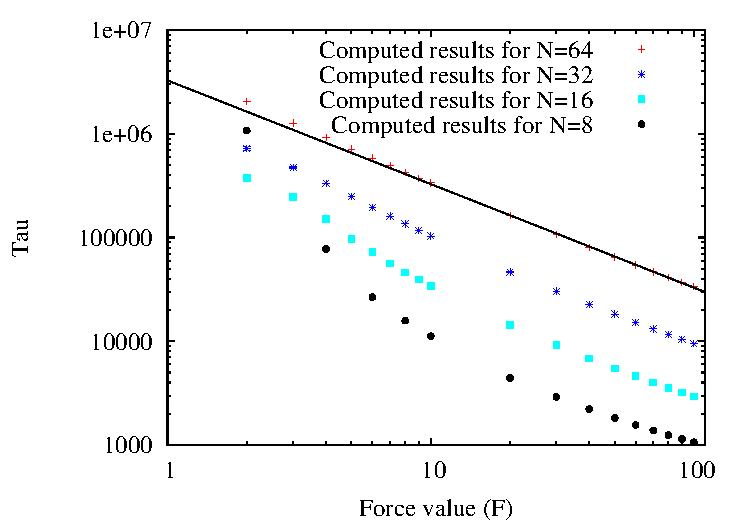
\includegraphics[width=0.48\textwidth]{translocfthinpore.pdf} 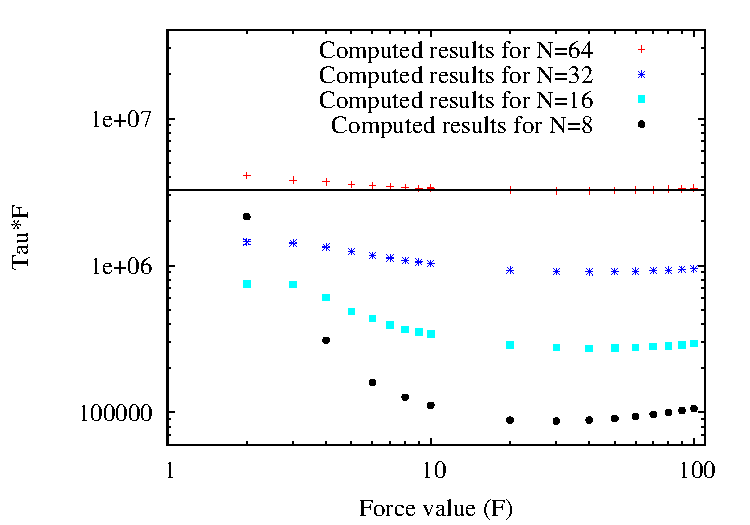
\includegraphics[width=0.48\textwidth]{translocthinpore.pdf}

\caption{Lors de la translocation à travers un nanopore étroit, la transition entre les les deux régimes observés précédemment semble se faire pour des forces plus élevées. Le frottement pourrait être caractérisé par une diminution de la force effective. La loi $\tau \propto N^{1+\nu}$ est toujours suivie. La modification de la barrière d'énergie introduit un comportement imprévu à gauche de la courbe. Le comportement anormal du cas $N=8$ à faible forces est dû a des effets de tailles finies et aux conditions de test lors des simulations.}
\label{thinpore}
\end{center}
\end{figure}

Les lois d'échelles ne semblent pas avoir été modifiées à fortes forces, si ce n'est en introduisant une force effective à cause du frottement. L'application d'une force faible sur un nanopore étroit permet de ralentir la translocation (Figure \ref{both}).

\begin{figure}[H]
\begin{center}
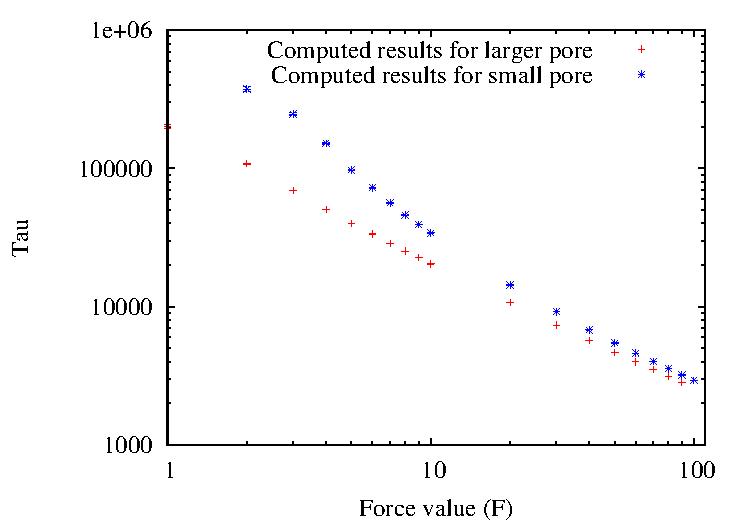
\includegraphics[width=0.45\textwidth]{translocporedifn.pdf} 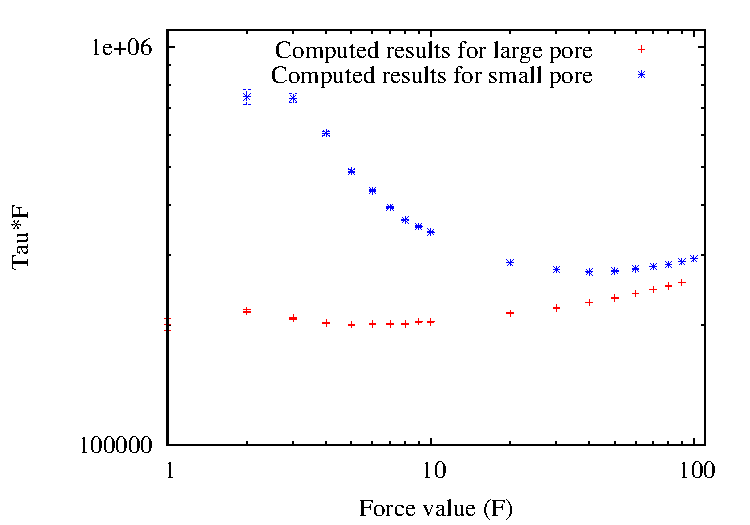
\includegraphics[width=0.45\textwidth]{translocporedif.pdf}

\caption{A forte force, l'étroitesse du pore ne modifie pas les lois d'échelles. A faible force la modification de la barrière énergétique entraine une augmentation importante du temps de translocation (ici $N=16$).}
\label{both}
\end{center}
\end{figure}

Nous allons maintenant nous intéresser à l'influence des propriétés vibrationnelles du graphène sur la translocation.

\subsubsection*{Translocation à travers un pore vibrant}

Pour les vibrations, nous avons choisi de thermaliser notre membrane a une température bien plus faible que celle du polymère ($0.005\epsilon$) afin de pouvoir observé l'échauffement du pore au cours de la translocation. Afin de conserver une trajectoire naturelle, nous avons imposé au potentiel harmonique des carbone une raideur adaptée. La Figure \ref{temperature} commente les résultats observés sur une translocation unique (en ce qui concerne les résultats ayant une signification statistique, nous obtenons des résultats surprenants montrés en annexe).
\begin{figure}[H]
\begin{center}
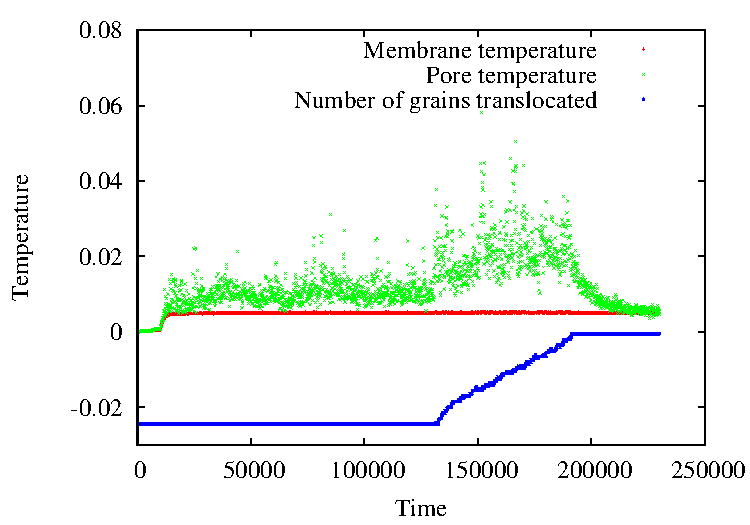
\includegraphics[width=0.49\textwidth]{tempmurmobil.pdf}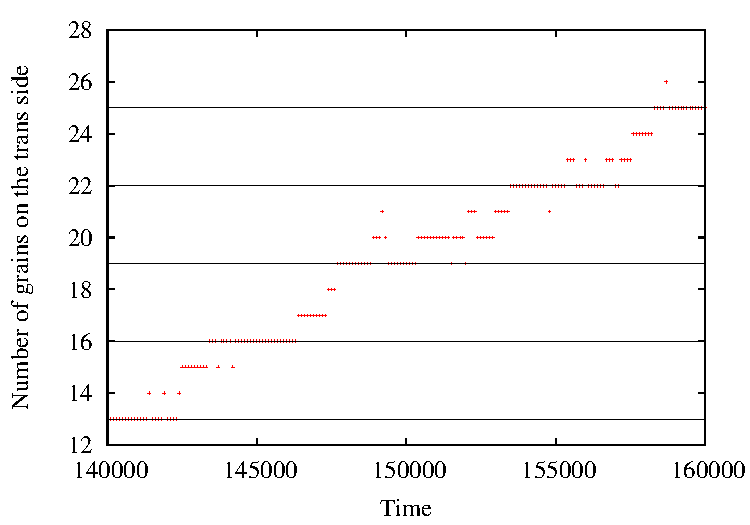
\includegraphics[width=0.49\textwidth]{murmobil.pdf}

\caption{A gauche: Evolution de la température de la membrane et du pore au cours de la thermalisation, suivie de la translocation, le nombre de grains passés du coté trans est donné de manière indicative (échelle arbitraire). Lors de la translocation, le polymère échauffe la paroi du pore, qui retourne à l'équilibre thermique une fois la translocation terminée. A droite: Illustration de la translocation ayant lieu par paliers, le gros grain latéral passant difficilement à travers le pore.}
\label{temperature}
\end{center}
\end{figure}




\section{Conclusion}

Au cours de ce stage, nous avons construit un modèle gros grains de polymère présentant des contraintes stérique comparables à celles de l'ADN. Notre approche est originale, en ce qu'elle consiste à créer un polymère suffisamment détaillé pour reproduire certains comportements de l'ADN, mais suffisamment simple pour vérifier des lois d'échelles prévues par la physique statistique. L'élaboration de ce polymère nous a permis d'évaluer des exposants critiques caractérisant la translocation.\\

Nous avons, dans un premier temps, vérifié la cohérence de notre modèle en retrouvant des résultats connus pour un polymère libre. Ces préliminaires effectués, nous avons trouvé les lois d'échelles régissant notre système, dans le cas d'un nanopore large, ainsi que dans celui, plus original, d'un nanopore étroit modifiant la barrière d'énergie entropique à franchir. Ceci nous a permis de montrer qu'il est possible, à faible forces dans un pore étroit, d'augmenter significativement le temps de translocation, condition préalable à un éventuel séquençage.\\

Ce travail est toujours en cours et sera poursuivie par une thèse dans l'équipe de Arnaud Buhot. Nous nous attacherons donc à mieux comprendre (et corriger si nécessaire) ce qui a été mis en œuvre pour le pore vibrant. En plus de la vibration du pore, nous modéliserons la flexibilité du plan de la membrane dans son ensemble. Enfin, l'utilisation d'une force de type électrique, agissant dans au sein du pore, ou encore un travail à vitesse imposée, pourront être envisagés.




\bibliography{biblio}
\bibliographystyle{ieeetr}




\end{document}

